\documentclass[11pt,a4paper]{article}

\usepackage{iftex}
\ifTUTeX
  \usepackage{fontspec}
  \setmainfont{texgyretermes}[Extension=.otf, UprightFont=*-regular, BoldFont=*-bold,
    ItalicFont=*-italic, BoldItalicFont=*-bolditalic]
\else
  \usepackage[T1]{fontenc}
  \usepackage[utf8]{inputenc}
\fi
\usepackage[margin=2.4cm]{geometry}
\usepackage{amsmath,amssymb}
\usepackage{booktabs}
\usepackage{tabularx}
\usepackage{array}
\usepackage{graphicx}
\usepackage{caption}
\usepackage{enumitem}
\usepackage[hidelinks]{hyperref}
\usepackage{xurl}
\emergencystretch=2em

\captionsetup{font=small,labelfont=bf}
\setlist{nosep,leftmargin=*}
\newcolumntype{L}{>{\raggedright\arraybackslash}X}
\newcommand{\code}[1]{\texttt{#1}}

\title{Downscaling GRACE/GRACE-FO water storage with a conditional diffusion model trained
  on paired GRACE and WaterGAP fields: a proposal}
\author{H. Oğuz Bolat}
\date{Proposal, draft for discussion\\[2pt] 18 November 2026}

\begin{document}
\maketitle

\begin{abstract}
\noindent
We propose a method for adding spatial detail to GRACE and GRACE-FO terrestrial water storage
(TWS) fields below the resolution of the observations. A conditional diffusion model receives
a GRACE field limited to spherical-harmonic degree 32 and generates the detail between degrees
32 and 128 (half-wavelengths from about 600\,km to 160\,km) as an ensemble. The detail is
learned from the WaterGAP hydrological model: the network is first trained on WaterGAP alone
and then fine-tuned on months for which both GRACE and WaterGAP are available, with GRACE as
input and WaterGAP's detail as target. The loss acts on the generated detail only, and a
consistency projection fixes all coarser coefficients to their GRACE values, so that the
observed large-scale field is preserved exactly. The proposal follows from two earlier
experiments, which showed that such detail cannot be inferred from coarser scales of GRACE
itself, and that a network trained on model fields alone performs well on GRACE but is
limited by the mismatch between model and observed inputs. We describe the method, the data,
a four-level evaluation ending with independent data over Türkiye, a staged experimental
plan, and the risks we have identified, and we list the points on which a decision is needed.
\end{abstract}

\section{Motivation}

GRACE and GRACE-FO resolve monthly mass change to a spatial scale of a few hundred
kilometres. Many hydrological applications require finer detail, and that detail cannot be
recovered from the observations themselves. A generative model conditioned on the observed
field can supply it as an ensemble of realisations that agree with the observation at the
scales it resolves, the ensemble spread expressing the uncertainty of what is added.

Two earlier experiments, documented in the progress report of 18 November 2026, determine
the form of the present proposal. In the first, a network was trained to add one octave of
spherical-harmonic detail at coarse scales, where GRACE resolves both input and target, and
was then applied one octave finer. It was the best method at its training scale but worse than
a spectral baseline one octave finer, on GRACE and on a hydrological model alike, whereas a
network trained at the finer scale itself performed well. Fine detail must therefore be learned
from examples at the scale concerned, which GRACE cannot provide below its resolution.

In the second experiment the examples were taken from hydrological models: a network was
trained on ten ISIMIP3a models, with the model field limited to a coarse degree as input and
the model's own finer detail as target, and was then applied to GRACE. At scales where GRACE
can serve as reference (degrees 8 to 16 and 16 to 32), it improved on the spectral baseline by
7--10\,mm in the continuous ranked probability score (CRPS) and reproduced a substantial part
of the observed detail. Its ensembles were, however, too narrow, and remained so after
calibration unless the calibration used GRACE itself, which is not possible at the target
scales. We attribute this to a mismatch of inputs: the network was trained on model fields
limited to a coarse degree and then received GRACE fields, which it had never seen and which
differ from model fields at large scales.

The method proposed here removes this mismatch by placing GRACE on the input side during
training.

\section{Proposed method}\label{sec:method}

\subsection{Task}
For a single month, the input is the GRACE TWS field limited to degree $L_\mathrm{in} = 32$,
and the output is an ensemble of fields limited to degree $L = 128$
(Figure~\ref{fig:bands}). Fields are limited with a cosine taper $w_L(l)$, equal to 1 up to
degree $0.8L$ and falling to 0 at degree $L$. No auxiliary inputs such as precipitation,
temperature or topography are used, so that the result depends on GRACE and on the learned
statistical relation only. Months are treated independently.

\begin{figure}[ht]
  \centering
  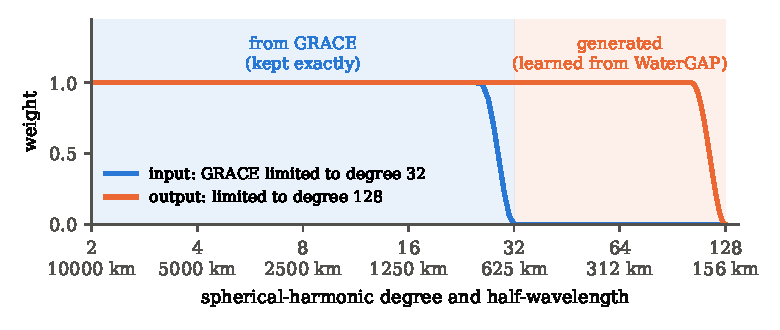
\includegraphics[width=0.72\linewidth]{figures/bands.pdf}
  \caption{Origin of the spectral content of the product. Degrees below 32 are taken from GRACE
  and are not altered; degrees from 32 to 128 are generated by the network, which learns them
  from WaterGAP.}
  \label{fig:bands}
\end{figure}

\subsection{Training target and loss}
The detail is learned from WaterGAP v2.2e. For a month with GRACE coefficients $g_{lm}$ and
WaterGAP coefficients $h_{lm}$, a combined set of coefficients is formed,
\begin{equation}
  c_{lm} =
  \begin{cases}
    g_{lm}, & l < L_\mathrm{in},\\
    h_{lm}, & l \ge L_\mathrm{in},
  \end{cases}
\end{equation}
from which the input $x_\mathrm{in} = w_{L_\mathrm{in}} c$ and the target
$x = w_L c$ are computed. The input is then exactly the GRACE field limited to
$L_\mathrm{in}$, and the detail $d = x - x_\mathrm{in}$ contains WaterGAP's signal at all
degrees from $L_\mathrm{in}$ upward. (It also contains the part of GRACE that the taper
removes between $0.8L_\mathrm{in}$ and $L_\mathrm{in}$, which is known from the input and is
restored exactly by the projection described below.) The network generates $d$, and the loss compares the
generated with the true detail. The coarse part of the field does not enter the loss.

This choice is deliberate. A loss on the complete field would reward the network for moving
GRACE's large-scale field towards the model, for instance by weakening a groundwater depletion
signal that GRACE observes and the model underestimates. With a loss on the detail, the product
is GRACE made sharper with model-like detail, not a hydrological model adjusted by GRACE.

\subsection{Consistency with the observation}
After generation, every coefficient of degree below $L_\mathrm{in}$ is replaced by its GRACE
value, recovered from the input as $x^{\mathrm{in}}_{lm} / w_{L_\mathrm{in}}(l)$. This is an
exact linear projection that leaves the true target unchanged. Limiting any output back to
degree $L_\mathrm{in}$ returns the input to numerical precision (of order $10^{-15}$\,mm in
our implementation), so GRACE alone determines the coarse part of the product.

\subsection{Generative model}
The network is the U-Net used in the earlier experiments (16.3 million parameters, without
attention, with padding that respects the periodicity in longitude and the continuity across
the poles). Fields are represented on global equiangular grids of $4L \times 8L$ points, each
map is divided by the area-weighted root mean square of its input, and each training sample is
rotated by a random rotation of the sphere, applied identically to input and target.

The diffusion model follows the EDM formulation, with the training noise distribution widened
relative to its default ($\ln\sigma \sim \mathcal N(-0.4, 1.6^2)$, $\sigma_\mathrm{max} = 20$);
the earlier experiments showed the default to be unsuitable for this problem. Samples are
drawn with the stochastic second-order sampler in 32 steps, which in our calibration tests
improved both accuracy and ensemble spread over the deterministic sampler. The ensemble mean
serves as the single best estimate.

A direct network with the same architecture, trained with a weighted squared error to predict
the detail in one pass, is trained alongside as a baseline. It yields the conditional mean
without uncertainty and shows what the diffusion formulation contributes.

\subsection{Training in two phases}
Months with both GRACE and WaterGAP are available only from April 2002 to December 2019,
which is a small sample for training a network of this size. Training therefore proceeds in
two phases. In the first, the network is trained on WaterGAP alone for 1901--1989 (validated
on 1990--2001), with the WaterGAP field limited to $L_\mathrm{in}$ as input and WaterGAP's
detail as target; here it learns the fine-scale structure of the model from more than a
thousand months. In the second, training continues on the paired months, with GRACE as input
and WaterGAP's detail as target, so that the network adapts to observed inputs. Training on
the paired months alone, and training on both kinds of sample simultaneously, are retained as
alternatives.

\subsection{Resolution}
The target is degree 128. Whether it is better reached in one step (32 to 128) or in two
single-octave steps (32 to 64 and 64 to 128) will be decided by experiment
(Section~\ref{sec:plan}). In the two-step variant only the first step receives GRACE directly;
the second is fine-tuned on the output of the first.

\section{Data}

\subsection{GRACE/GRACE-FO}
The input fields are derived from the ITSG-Grace2018 and ITSG-Grace\_operational monthly
solutions (260 months from April 2002 to September 2026), with $C_{20}$ and $C_{30}$ replaced
by the TN-14 values, glacial isostatic adjustment removed with the model of Caron et~al.\
(2018), and anomalies taken relative to 2004--2009 and expressed as equivalent water height;
degrees 0 and 1 are excluded. Both an unfiltered and a DDK5-filtered version are available.
Since WaterGAP contains no ocean signal and does not represent the ice sheets, the GRACE fields
are set to zero over the ocean, Greenland and Antarctica before use, so that input and target
share a domain.

\subsection{WaterGAP}
The target is monthly TWS from WaterGAP v2.2e (GSWP3-W5E5 forcing, historical human water
use) for 1901--2019 at $0.5^\circ$, expanded to degree 128. Cells whose storage drifts by more
than 1\,m over the simulation (unbounded snow accumulation on glaciers and point-like urban
groundwater abstraction, about 2600 cells) are set to zero anomaly. Anomalies are referred to
2004--2009 as for GRACE.

\subsection{Data used for comparison}
The GLWS2.0 data set (Gerdener et~al.\ 2023), obtained by assimilating GRACE and GRACE-FO into
WaterGAP, is the existing product closest in purpose to ours and will serve as a benchmark.
Because it is derived from the same two sources, agreement with it is in part expected by
construction, and we do not regard it as an independent validation. The comparison will be
made at a common resolution, with GLWS limited to our target degree.

Nine further ISIMIP3a models (CWatM, H08, HydroPy, JULES-ES, JULES-W2, LPJmL, MIROC-INTEG-LAND,
ORCHIDEE-MICT and WEB-DHM-SG), prepared in the same way as WaterGAP, are retained for
comparison but are not used as training targets.

\subsection{Masks and data splits}
A region over Türkiye (30--45$^\circ$N, 20--50$^\circ$E), enlarged by one half-wavelength of
the target degree, is excluded from all training and reserved for the final test. Greenland
and Antarctica are excluded from the loss and the scores, and scores are computed over land.
The data are divided into contiguous blocks of months (Table~\ref{tab:splits}). The gap
between the GRACE and GRACE-FO missions separates the validation from the test period, which
also shows whether the method carries over to GRACE-FO. GRACE-FO months after 2019 have no
target and are the period to which the finished product is applied.

\begin{table}[ht]
\centering\small
\caption{Data splits.}
\label{tab:splits}
\begin{tabular}{llll}
  \toprule
  data & use & period & months \\
  \midrule
  WaterGAP alone & first training phase & 1901--1989 & 1068 \\
  WaterGAP alone & validation of the first phase & 1990--2001 & 144 \\
  GRACE and WaterGAP & second training phase & 2002-04 to 2014-12 & 140 \\
  GRACE and WaterGAP & validation & 2015-01 to 2017-06 & 22 \\
  GRACE-FO and WaterGAP & test & 2018-06 to 2019-12 & 17 \\
  \bottomrule
\end{tabular}
\end{table}

\section{Evaluation}\label{sec:eval}

The principal score is the CRPS, computed with the fair ensemble estimator; it rewards both
accuracy and appropriate spread. We further report the root mean square error and the
correlation of the ensemble mean, the ratio of ensemble spread to ensemble-mean error (1 for a
calibrated ensemble), and the coverage of the central 50\% and 90\% ensemble intervals. Methods
are compared through per-month CRPS differences with intervals from a moving-block bootstrap.
The reference methods are the input without added detail, a spectral baseline that adds random
detail with a power-law spectrum extrapolated from the input, its variant with the mean
spectrum of the training months, and the direct network.

The evaluation has four levels of increasing strength.

The first level scores the generated detail against WaterGAP's detail on the held-out paired
months. It establishes that the network has learned its task and that its spread is calibrated
with respect to the model, but not that the detail is real.

The second level repeats the complete procedure at coarser scales (degrees 8 to 16 and 16 to
32), where GRACE resolves the detail, and scores the output against the detail GRACE actually
observed. This is the only global test against observations. It measures how closely
WaterGAP-like detail, added to a GRACE field, resembles reality at scales where this can be
checked.

The third level compares the product with GLWS2.0 at the target scales and reports where the
two agree and where they differ, without a criterion of success.

The fourth level compares the product over the Türkiye test region with data that involve
neither GRACE nor WaterGAP, such as groundwater levels, GNSS loading displacements or basin
water budgets. It is the only test of the generated detail against independent observations,
and the data for it remain to be identified.

For the first and second levels, the method is regarded as successful if it improves on the
baselines and on the direct network in CRPS, with a bootstrap interval excluding zero, and has
a spread-to-error ratio between 0.85 and 1.15. For the fourth level, the product should agree
with the independent data more closely than GRACE at its native resolution, and preferably at
least as closely as WaterGAP and GLWS2.0. The test months and the test region will not be used
until the design is fixed.

\section{Experimental plan}\label{sec:plan}

The work is arranged in three stages, so that the design is tested where it is inexpensive
before the costly runs are made.

Stage 1 applies the method at coarse scales (degrees 8 to 32), on grids that the available
workstation handles within hours and where the second evaluation level is available. Its
variants (Table~\ref{tab:stage1}) answer whether the paired fine-tuning improves on the
earlier model-only training, whether one step or two is preferable, whether the first training
phase is needed, and whether the diffusion model improves on the direct network. The code for
this stage has been written and tested, and the first runs are in progress.

\begin{table}[ht]
\centering\small
\caption{Variants of stage 1, all scored at levels one and two of Section~\ref{sec:eval}.}
\label{tab:stage1}
\begin{tabularx}{0.92\linewidth}{lLL}
  \toprule
  & variant & question \\
  \midrule
  A & first phase only (trained on model fields) & reference: the earlier approach \\
  B & both phases, two steps (8 to 16, 16 to 32) & does the paired phase help? \\
  C & both phases, one step (8 to 32) & one step or two? \\
  D & paired months only & is the first phase needed? \\
  E & direct network, trained as B & does the diffusion model help? \\
  \bottomrule
\end{tabularx}
\end{table}

Stage 2 takes the best variant to the target scales (degrees 32 to 128) and evaluates it at
levels one and three. Global grids at degree 128 do not fit the memory of the workstation
(32\,GB) at a useful batch size, so this stage requires training on sub-regions of the grid,
which has yet to be implemented.

Stage 3 is the comparison with independent data over Türkiye (level four), followed by the
application to the GRACE-FO months after 2019.

\section{Risks and limitations}

The fine-scale content of the product is that of WaterGAP. Where the model lacks a process or
misplaces a signal, the generated detail inherits the deficiency, and where GRACE observes a
large-scale signal that the model does not contain, the signal is preserved but not sharpened.
The ensemble spread expresses the ambiguity of the detail given the GRACE field under the
assumption that WaterGAP's fine-scale behaviour is correct; it does not include the model's
own errors. In the earlier experiment, training on ten models gave better agreement with GRACE
than training on WaterGAP alone (24.0 against 28.0\,mm at degrees 8 to 16), and the use of
several models as targets may be reconsidered once the paired design is established.

GRACE and WaterGAP differ in amplitude at scales where both carry signal. In a preliminary
comparison over six validation months, the root mean square of GRACE's detail over land was
two to three times that of WaterGAP's (60 against 31\,mm at degrees 8 to 16; 106 against 35\,mm at
degrees 16 to 32; the GRACE fields in this comparison were not yet restricted to land and so
include leakage from the ocean and the ice sheets). A network
trained towards WaterGAP's detail will therefore add less variability than GRACE observes at
these scales, which will count against it at the second evaluation level. How much of the
difference is signal absent from the model (glaciers, groundwater trends), how much is
leakage, and how much is observational noise is not yet known; stage 1 is designed to
quantify its effect.

The paired sample is small: 140 months for training, 22 for validation and 17 for testing.
Random rotations multiply the training samples but not the hydrological situations they
contain, so overfitting in the second phase is the principal technical risk, and the short
validation and test periods will give wide confidence intervals.

Finally, the comparison with GLWS2.0 cannot establish correctness, for the reason given above,
and the strength of the final validation depends on independent data for Türkiye that have
not yet been secured.

\section{Points for decision}

\begin{enumerate}
  \item Independent data for the Türkiye region (groundwater levels, GNSS loading, basin
    water budgets, regional products) for the fourth evaluation level.
  \item The GRACE product and filter used as input: ITSG with DDK5 filtering, or unfiltered.
  \item The target resolution: degree 128 (about 160\,km), or finer at a later stage.
  \item WaterGAP as the sole training target, or several hydrological models.
  \item The treatment of the amplitude difference between GRACE and WaterGAP, should stage 1
    show it to be limiting.
\end{enumerate}

\end{document}
